\documentclass[12pt]{article}
\usepackage{amsmath}
\usepackage{hyperref}
\usepackage{mathtools}
\usepackage{amsfonts}
\usepackage{lastpage}
\usepackage{tikz}
\usepackage{pdfpages}
\usepackage{gauss}
\usepackage{fancyvrb}
\usepackage{fancyhdr}
\usepackage{graphicx}
\pagestyle{fancy}
\fancyfoot[C]{\footnotesize Page \thepage\ of 5}
\DeclareGraphicsExtensions{.pdf,.png,.jpg}
\title{Database and Web Programming}
\author{Nikolaj Dybdahl Rathcke}
\chead{Nikolaj Dybdahl Rathcke - rfq695}

\begin{document}

\section*{1: Indexing}
Construct a B+tree for the following set of key values:\\
$$(88, 84, 65, 67, 86, 75, 76, 77, 83, 71, 85, 90, 80)$$
Assume that the tree is initially empty and that keys are added in the given order. The number of keys that can fit in each node is three. Show the tree after insertion of each of the values.\\
\\
Insertion of 88:\\
$$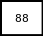
\includegraphics[scale=0.5]{1}$$
Insertion of 84:\\
$$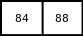
\includegraphics[scale=0.5]{2}$$
Insertion of 65:\\
$$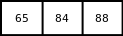
\includegraphics[scale=0.5]{3}$$
Insertion of 67:\\
$$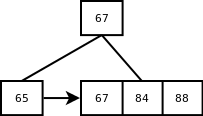
\includegraphics[scale=0.5]{4}$$
Insertion of 86:\\
$$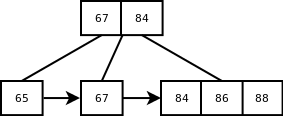
\includegraphics[scale=0.5]{5}$$
Insertion of 75:\\
$$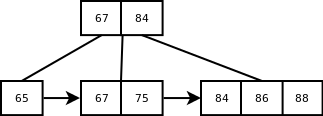
\includegraphics[scale=0.5]{6}$$
Insertion of 76:\\
$$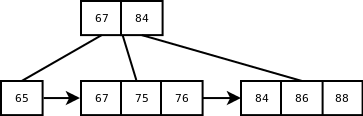
\includegraphics[scale=0.5]{7}$$
Insertion of 77:\\
$$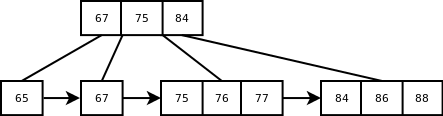
\includegraphics[scale=0.5]{8}$$
Insertion of 83:\\
$$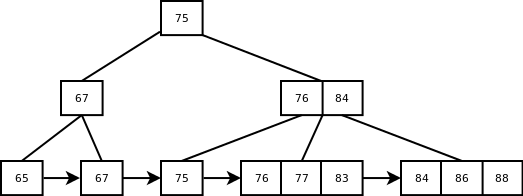
\includegraphics[scale=0.5]{9}$$
Insertion of 71:\\
$$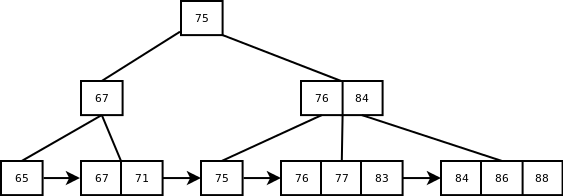
\includegraphics[scale=0.5]{10}$$
Insertion of 85:\\
$$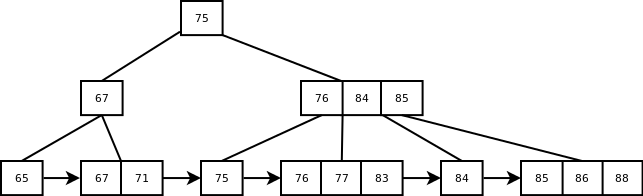
\includegraphics[scale=0.5]{11}$$
Insertion of 90:\\
$$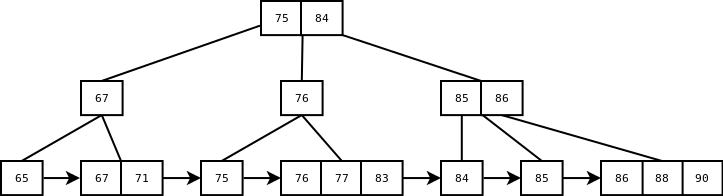
\includegraphics[scale=0.5]{12}$$
Insertion of 80:\\
$$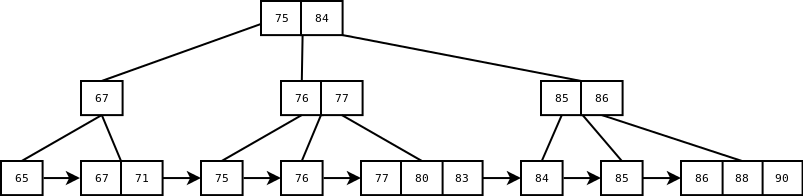
\includegraphics[scale=0.5]{13}$$
Which is the final tree after all the key values have been inserted.

\section*{2: Web application}
The URL's are:\\
\\
\url{http://dbw.diku.dk/~rfq695/problem2\_show\_orders.php}\\
\\
For the other 2, there is no URL such as:\\
\\
http://dbw.diku.dk/~rfq695/problem2\_view\_order.php\\
http://dbw.diku.dk/~rfq695/problem2\_view\_customer.php\\
\\
Since these needs to be given with an id, either ordernumber or customernumber. But the links from the first link will lead to valid sites.

\section*{3: Web application and Transactions}
The URL for 'add product' are:\\
\\
\url{http://dbw.diku.dk/~rfq695/problem3\_add\_product.php}\\
\\
To which the site:\\
\\
http://dbw.diku.dk/$\sim$rfq695/problem3\_added.php\\
\\
is where the information is send to and is added to the database, after which it redirects back to the original page.\\
\\
For 'update product', the URL is:\\
\\
\url{http://dbw.diku.dk/~rfq695/problem3\_update\_product.php}\\
\\
Note: I haven't included the form with information about the product on the page since I found it would be a waste. The form appears when the code for a product is clicked.
The site:\\
\\	
http://dbw.diku.dk/$\sim$rfq695/problem3\_updated.php\\
\\
functions in the same way as mentioned in 'problem3\_added.php'.

\section*{4: Database Programming and XML}
\subsection*{1}
The Java file and the xml file is located in the problem 4 folder.

\subsection*{2}
Make the XPath expressions that will answer the following questions on the XMLSchema and XML file from Problem 4.1:\\
\\
a. Get all order numbers\\
\\
/orders/order/@number\\
\\
b. Get the customername of all orders with “In Process” status\\
\\
/orders/order[@status="In Process"]/@customername\\
\\
c. Get the productnames from orders created on 2005-05-29\\
\\
/orders/order[@date="2005-05-29"]/orderdetail/@productname

\subsection*{3}
The SQL file is located in the problem 4 folder.

\end{document}